\documentclass[final,3p,times]{elsarticle}

\usepackage{amsmath}
\usepackage{amssymb}
\usepackage{booktabs}
\usepackage{graphicx}
\usepackage{subcaption}
\usepackage{siunitx}
\usepackage{url}

\journal{AI4E Coursework: Artificial Intelligence for Energy Engineering}

\begin{document}

\begin{frontmatter}

\title{Coursework: Surrogati DeepCFD Physics-Informed per Flusso Interno 2D}

\author{Ivan Brillo}
\author{Luca BIundo}
\author{Andrea Di Matteo}
\author{Leonardo Magnolfi}

\affiliation{organization={AI4E Coursework Team, Artificial Intelligence for Energy Engineering},
             city={Italy},
             country={Italy}}

\begin{abstract}
Questo report presenta il confronto tra modelli surrogati DeepCFD per la previsione stazionaria di flussi 2D in canali con ostacolo. Sono state analizzate quattro famiglie di modelli (Base, Attention, FNO, Transformer), ciascuna valutata in regime solo dati e dati+fisica. La loss fisica segue una formulazione PINN con componenti di continuita', quantita' di moto e vincoli al bordo.

Nel budget di training usato in questo progetto, il modello con il miglior compromesso tra accuratezza e coerenza fisica e' UNet-Attention + physics, che migliora la MSE test masked di +8.25\% rispetto alla versione data-only. Il report include analisi quantitative, analisi per canale, confronto visuale in inferenza e discussione dei limiti osservati.
\end{abstract}

\end{frontmatter}

\section{Introduzione}
L'obiettivo del lavoro e' valutare quanto l'informazione fisica possa migliorare i surrogati neurali per CFD rispetto a una configurazione supervisionata classica. Il confronto e' stato impostato in modo controllato: stesso split dati, stessa pipeline di valutazione e stesso budget di training per tutte le architetture.

Sono stati valutati due regimi:
\begin{itemize}
    \item \textbf{data-only}: ottimizzazione solo sul fitting dei campi,
    \item \textbf{data+physics}: fitting dei campi con penalizzazione dei residui fisici.
\end{itemize}

\section{Impostazione sperimentale}
\subsection{Dati e metriche}
Gli input rappresentano geometria e condizioni al contorno su griglia fissa; i target sono $(U_x, U_y, p)$. Il dataset e' suddiviso in train/validation/test con rapporto 70/15/15.

Le metriche sono calcolate solo nel dominio fluido (masking dell'ostacolo), cosi' da evitare errori non fisicamente significativi nella regione solida.

\subsection{Architetture considerate (una alla volta)}
In tutti i casi la struttura generale e' encoder-decoder di tipo U-Net. Cambia il meccanismo interno di fusione e propagazione dell'informazione.

\subsubsection*{1) UNet-Attention}
Questa variante applica attention gates nelle skip connection. In pratica filtra le feature dell'encoder prima della fusione nel decoder, con l'obiettivo di enfatizzare regioni rilevanti del campo fluido.

\begin{figure}[h]
    \centering
    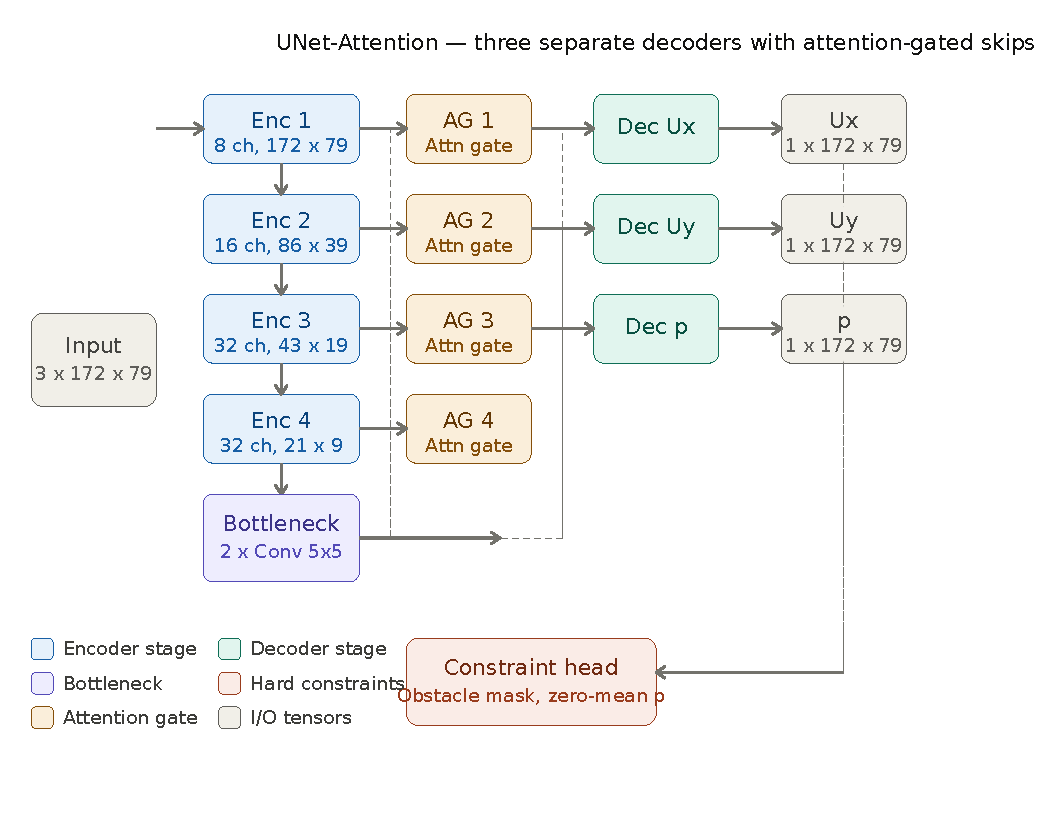
\includegraphics[width=0.9\linewidth]{figures/unet_attention_architecture.pdf}
    \caption{Architettura UNet-Attention.}
    \label{fig:arch_attn}
\end{figure}

\subsubsection*{2) UNet-FNO}
Questa variante sostituisce il bottleneck convoluzionale con un blocco in dominio di Fourier. L'idea e' modellare in modo piu' diretto dipendenze globali e strutture a lungo raggio.

\begin{figure}[h]
    \centering
    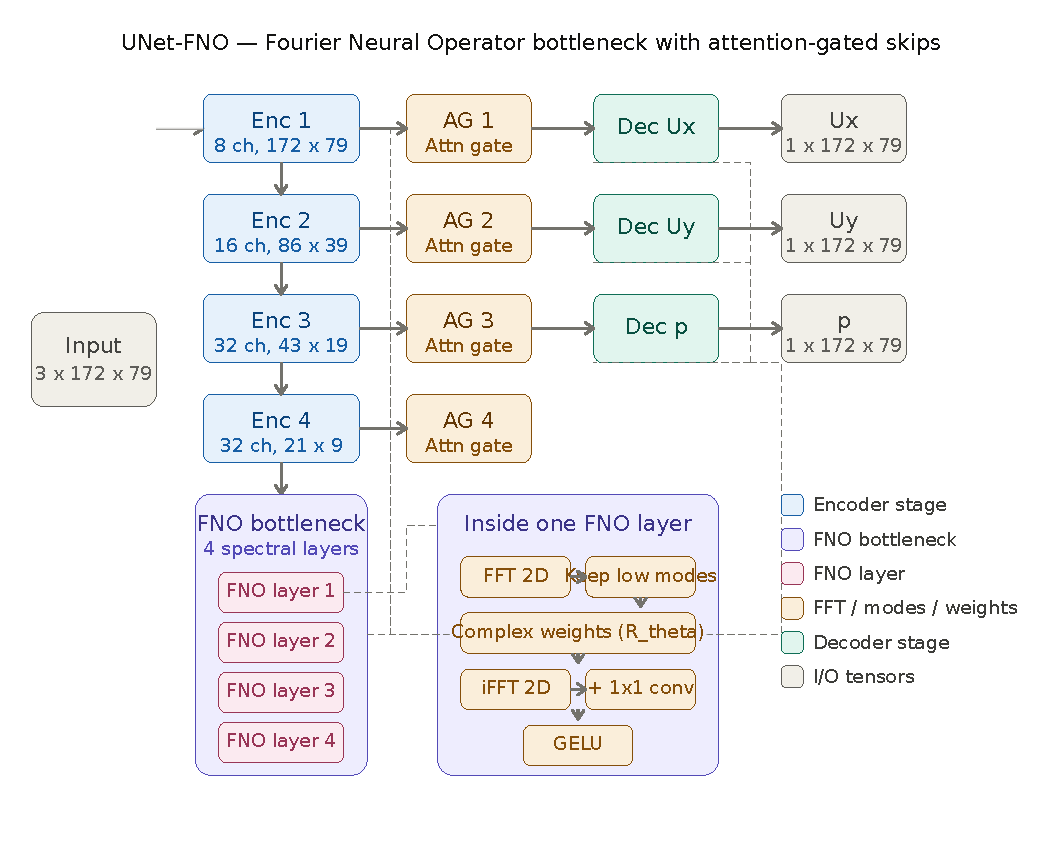
\includegraphics[width=0.9\linewidth]{figures/unet_fno_architecture.pdf}
    \caption{Architettura UNet-FNO.}
    \label{fig:arch_fno}
\end{figure}

\subsubsection*{3) UNet-Transformer}
Questa variante usa self-attention multi-head nel bottleneck, con interazioni globali adattive al contenuto delle feature latenti.

\begin{figure}[h]
    \centering
    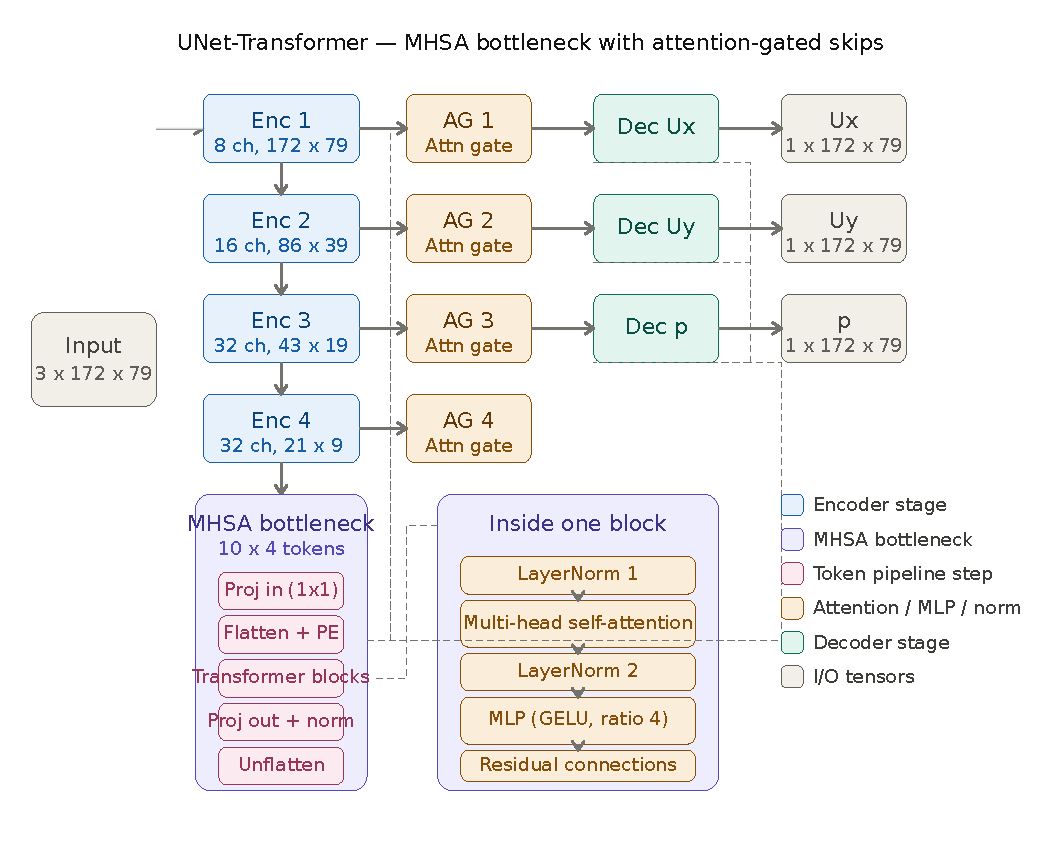
\includegraphics[width=0.9\linewidth]{figures/unet_transformer_architecture.pdf}
    \caption{Architettura UNet-Transformer.}
    \label{fig:arch_trans}
\end{figure}

\subsubsection*{4) UNet-Base (riferimento)}
La baseline mantiene un bottleneck convoluzionale standard ed e' usata come riferimento per confronto su accuratezza e costo computazionale.

\begin{table}[h]
\centering
\caption{Complessita' dei modelli considerati.}
\label{tab:arch_details}
\begin{tabular}{lc}
\toprule
Modello & Parametri \\
\midrule
UNet-Base & 518,051 \\
UNet-Attention & 526,115 \\
UNet-FNO & 577,379 \\
UNet-Transformer & 884,931 \\
\bottomrule
\end{tabular}
\end{table}

\subsection{Loss PINN e sue componenti}
La loss totale e' data da:
\begin{equation}
\mathcal{L}=\mathcal{L}_{data}+\lambda_{eff}(e)\,\mathcal{L}_{phys}.
\end{equation}

Il termine dati e' una combinazione pesata tra errori su $U_x$, $U_y$ e $p$:
\begin{equation}
\mathcal{L}_{data} = \frac{1}{3}\left(\frac{\mathrm{MSE}(U_x)}{w_{Ux}} + \frac{\mathrm{MSE}(U_y)}{w_{Uy}} + \frac{\mathrm{MAE}(p)}{w_p}\right).
\end{equation}

Il termine fisico e' composto da tre contributi:
\begin{equation}
\mathcal{L}_{phys}=\lambda_c\mathcal{L}_{cont}+\lambda_m\mathcal{L}_{mom}+\lambda_b\mathcal{L}_{bc},
\end{equation}
dove:
\begin{itemize}
    \item $\mathcal{L}_{cont}$ penalizza il residuo di continuita',
    \item $\mathcal{L}_{mom}$ penalizza i residui delle equazioni della quantita' di moto,
    \item $\mathcal{L}_{bc}$ penalizza la violazione delle condizioni al bordo.
\end{itemize}

Scelte operative adottate nel progetto:
\begin{itemize}
    \item residui calcolati solo nel dominio fluido,
    \item gauge correction della pressione (media nulla nel dominio fluido),
    \item attivazione progressiva del peso fisico durante il training.
\end{itemize}

\section{Risultati quantitativi}
\subsection{Confronto generale}
La Tabella~\ref{tab:main} riporta il confronto principale sul test masked. La migliore configurazione e' UNet-Attention (+phys).

\begin{table}[h]
\centering
\caption{Prestazioni sul test masked (solo dominio fluido). Valori piu' bassi sono migliori.}
\label{tab:main}
\begin{tabular}{lcc}
\toprule
Modello & MSE$_{tot}$ & SSE$_{tot}$ \\
\midrule
UNet-Base (data) & 1.0012e-4 & 3.9596 \\
UNet-Attention (data) & 1.0506e-4 & 4.1578 \\
UNet-FNO (data) & 1.2947e-4 & 5.1127 \\
UNet-Transformer (data) & 1.0226e-4 & 4.0446 \\
UNet-Attention (+phys) & \textbf{9.6396e-5} & \textbf{3.8139} \\
UNet-FNO (+phys) & 1.5376e-4 & 6.0683 \\
UNet-Transformer (+phys) & 1.0863e-4 & 4.2937 \\
\bottomrule
\end{tabular}
\end{table}

Variazione passando da data-only a data+physics:
\begin{itemize}
    \item UNet-Attention: +8.25\% (miglioramento),
    \item UNet-FNO: -18.76\% (peggioramento),
    \item UNet-Transformer: -6.24\% (peggioramento).
\end{itemize}

\subsection{Analisi per canale}
La Tabella~\ref{tab:channels} mostra la decomposizione per canale. In generale, la pressione pesa molto sulla MSE totale e $U_y$ risulta il canale piu' semplice.

\begin{table}[h]
\centering
\caption{MSE di test masked per canale (solo dominio fluido).}
\label{tab:channels}
\begin{tabular}{lccc}
\toprule
Modello & MSE$_{Ux}$ & MSE$_{Uy}$ & MSE$_p$ \\
\midrule
UNet-Base (data) & 4.7009e-05 & 6.7207e-06 & 2.4663e-04 \\
UNet-Attention (data) & 3.3783e-05 & 7.3448e-06 & 2.7406e-04 \\
UNet-FNO (data) & 1.3338e-04 & 8.9318e-06 & 2.4611e-04 \\
UNet-Transformer (data) & 4.6949e-05 & 7.6027e-06 & 2.5222e-04 \\
UNet-Attention (+phys) & 3.8904e-05 & \textbf{4.2500e-06} & \textbf{2.4603e-04} \\
UNet-FNO (+phys) & 2.0204e-04 & 1.1916e-05 & 2.4733e-04 \\
UNet-Transformer (+phys) & 7.0695e-05 & 7.7878e-06 & 2.4742e-04 \\
\bottomrule
\end{tabular}
\end{table}

\subsection{Convergenza e distribuzioni}
\begin{figure}[h]
    \centering
    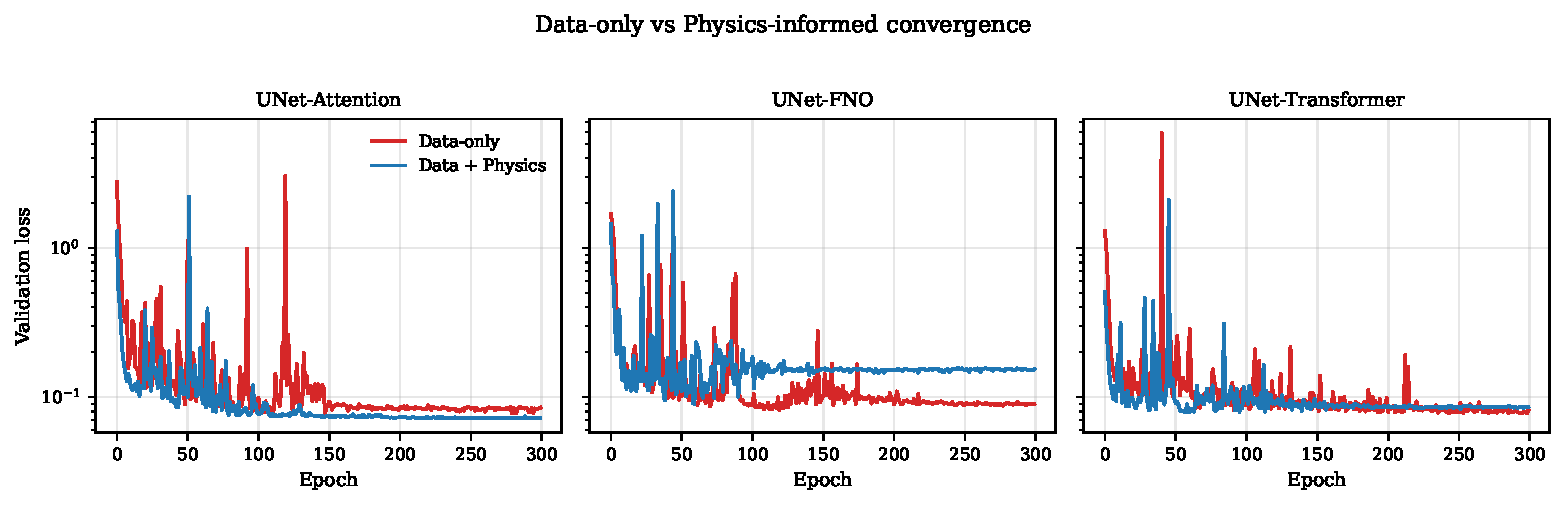
\includegraphics[width=0.95\linewidth]{figures/fig_data_vs_physics_curves.pdf}
    \caption{Convergenza in validation: confronto data-only vs data+physics.}
    \label{fig:curves}
\end{figure}

\begin{figure}[h]
    \centering
    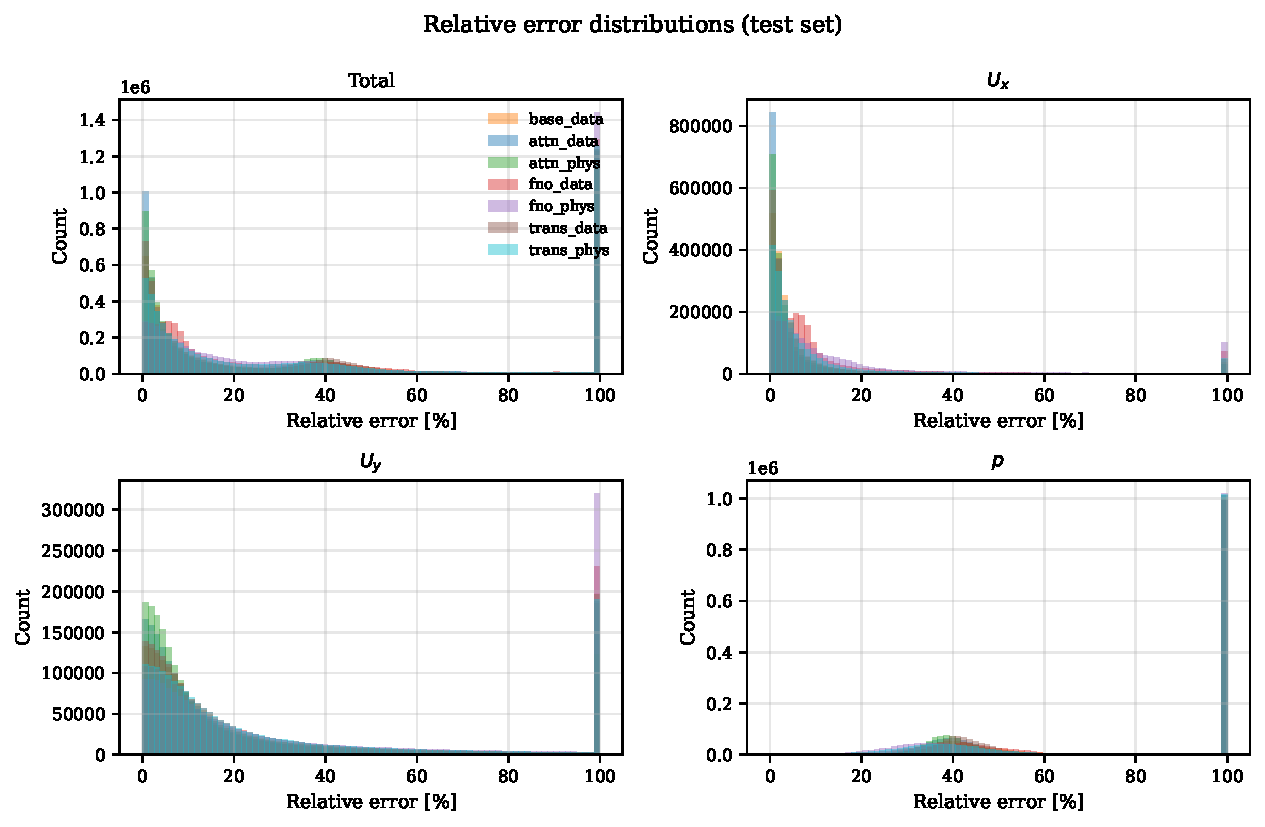
\includegraphics[width=0.95\linewidth]{figures/fig_relative_errors.pdf}
    \caption{Distribuzioni dell'errore relativo per canale e per modello.}
    \label{fig:relerr}
\end{figure}

\subsection{Costo di inferenza}
I surrogati risultano ordini di grandezza piu' veloci della baseline CFD di riferimento. La Tabella~\ref{tab:inference} riassume i tempi principali.

\begin{table}[h]
\centering
\caption{Sintesi dei tempi di inferenza dal benchmark.}
\label{tab:inference}
\begin{tabular}{lcc}
\toprule
Modello & Tempo campione (bs=1) [s] & Speedup (bs=100) \\
\midrule
UNet-Base (data) & 3.0546e-03 & 131,676 \\
UNet-Attention (data) & 5.9986e-03 & 97,067 \\
UNet-FNO (data) & 7.4316e-03 & 96,663 \\
UNet-Transformer (data) & 6.8713e-03 & 106,111 \\
UNet-Attention (+phys) & 5.9907e-03 & 96,906 \\
UNet-FNO (+phys) & 7.4206e-03 & 96,478 \\
UNet-Transformer (+phys) & 6.8762e-03 & 106,205 \\
\bottomrule
\end{tabular}
\end{table}

\section{Confronto visuale (solo figure presenti)}
Le figure seguenti sono tutte presenti nella cartella locale del report e mostrano il confronto qualitativo in inferenza.

\begin{figure}[h]
    \centering
    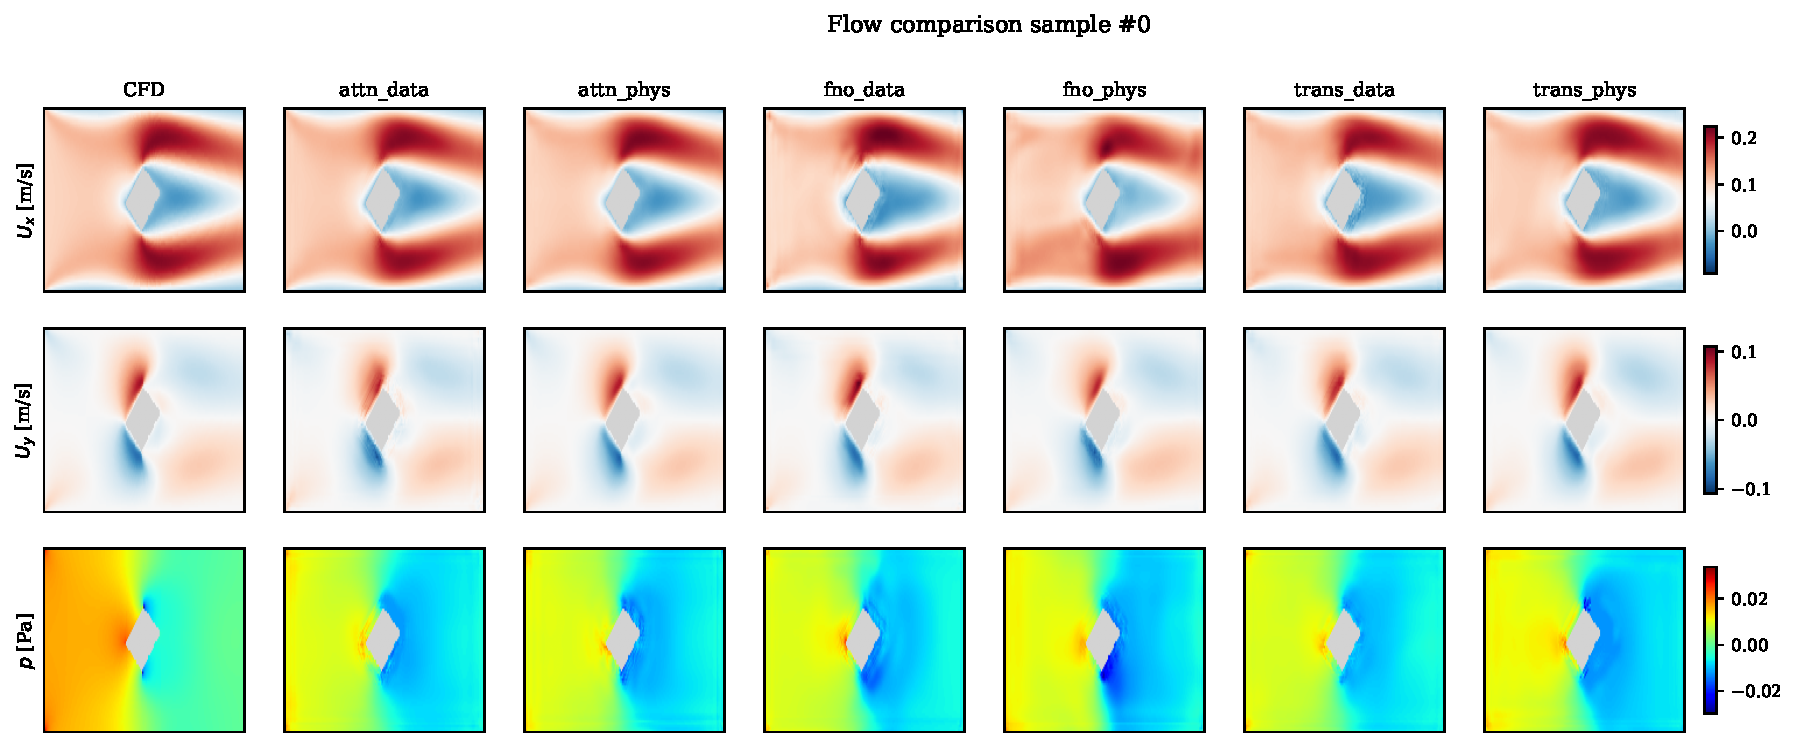
\includegraphics[width=0.95\linewidth]{figures/fig_flow_compare_data_phys_sample_0.pdf}
    \caption{Confronto data-only vs data+physics su campione 0.}
    \label{fig:flow0}
\end{figure}

\begin{figure}[h]
    \centering
    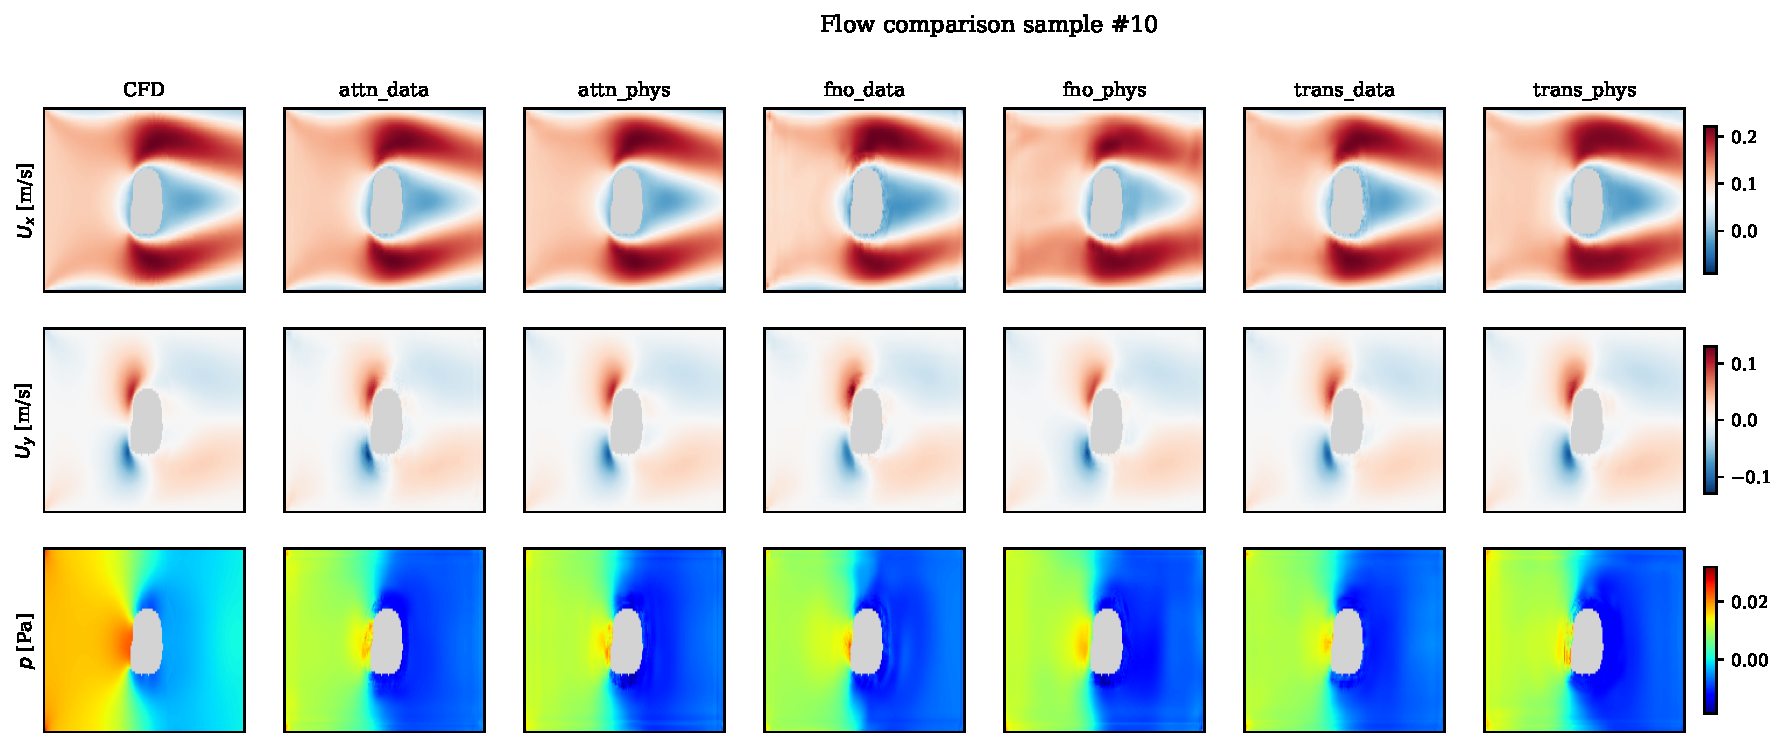
\includegraphics[width=0.95\linewidth]{figures/fig_flow_compare_data_phys_sample_10.pdf}
    \caption{Confronto data-only vs data+physics su campione 10.}
    \label{fig:flow10}
\end{figure}

\begin{figure}[h]
    \centering
    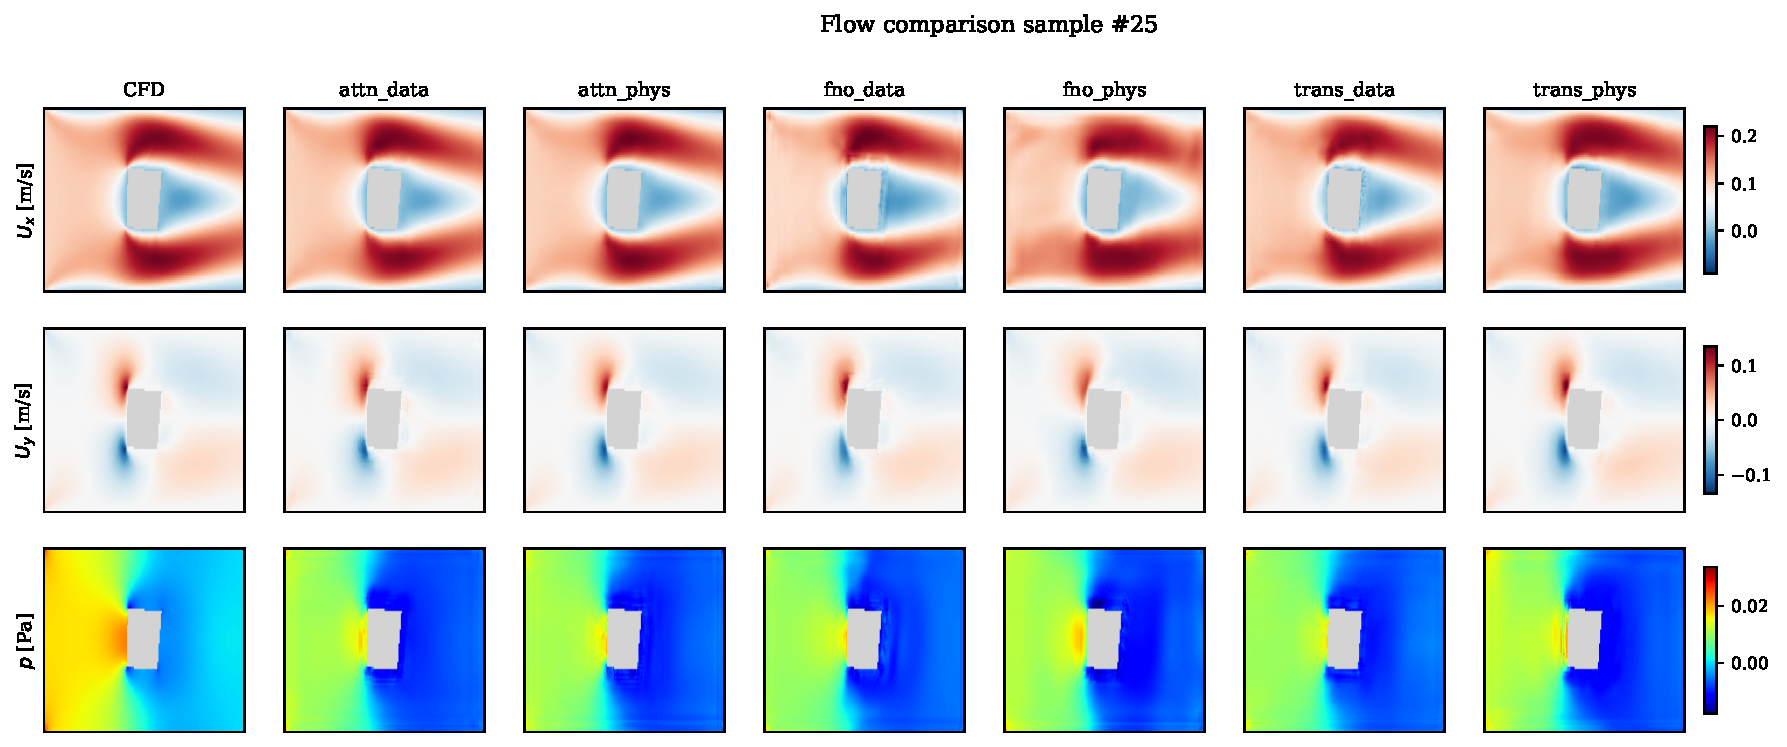
\includegraphics[width=0.95\linewidth]{figures/fig_flow_compare_data_phys_sample_25.pdf}
    \caption{Confronto data-only vs data+physics su campione 25.}
    \label{fig:flow25}
\end{figure}

\begin{figure}[h]
    \centering
    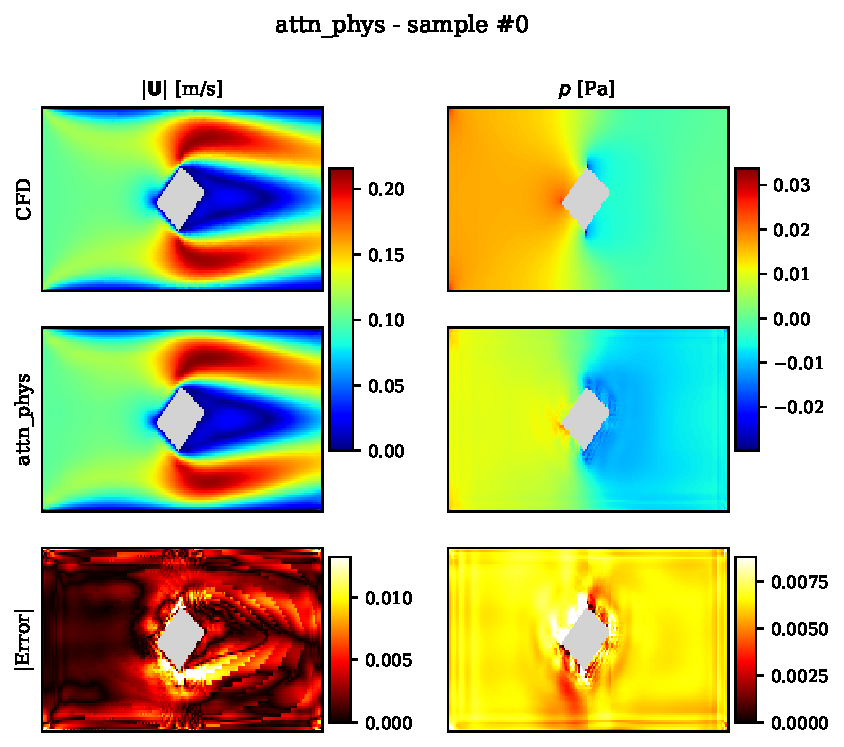
\includegraphics[width=0.95\linewidth]{figures/fig_umag_p_error_attn_phys_sample0.pdf}
    \caption{Mappe errore (modulo velocita' e pressione): UNet-Attention (+phys).}
    \label{fig:err_attn}
\end{figure}

\begin{figure}[h]
    \centering
    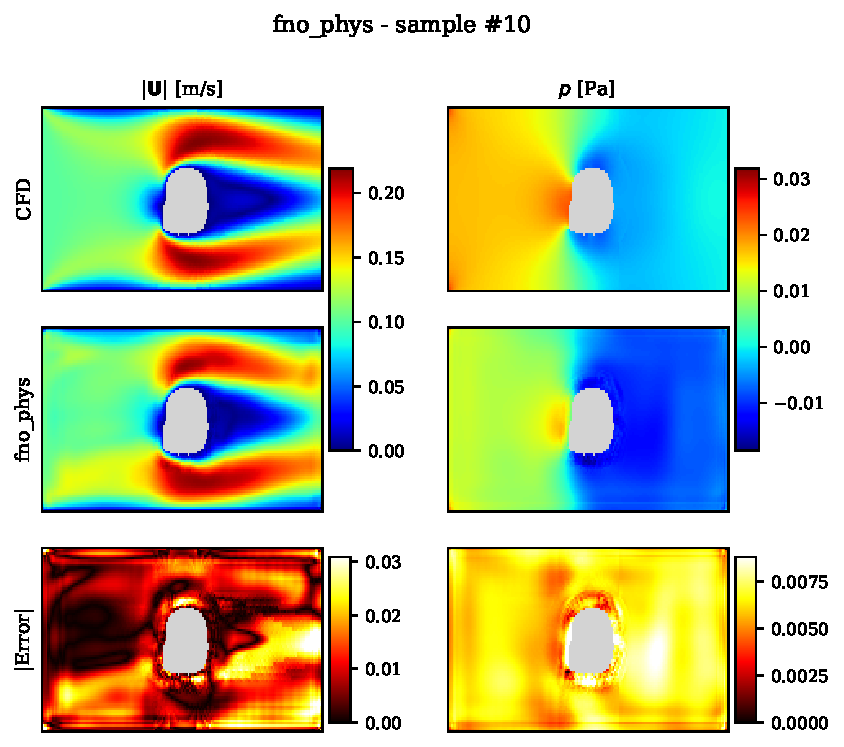
\includegraphics[width=0.95\linewidth]{figures/fig_umag_p_error_fno_phys_sample10.pdf}
    \caption{Mappe errore (modulo velocita' e pressione): UNet-FNO (+phys).}
    \label{fig:err_fno}
\end{figure}

\begin{figure}[h]
    \centering
    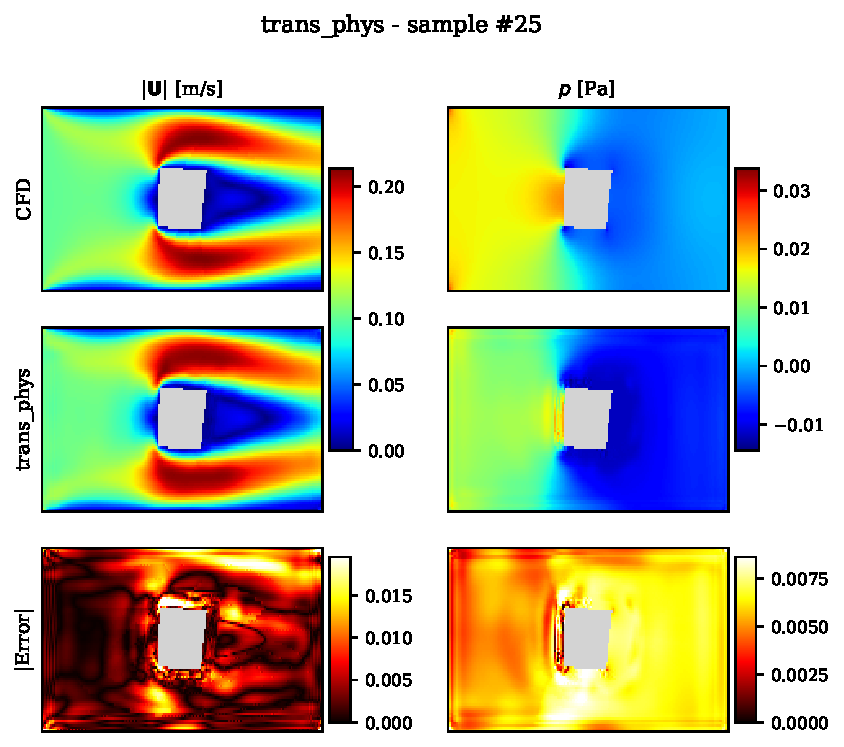
\includegraphics[width=0.95\linewidth]{figures/fig_umag_p_error_trans_phys_sample25.pdf}
    \caption{Mappe errore (modulo velocita' e pressione): UNet-Transformer (+phys).}
    \label{fig:err_trans}
\end{figure}

\begin{figure}[h]
    \centering
    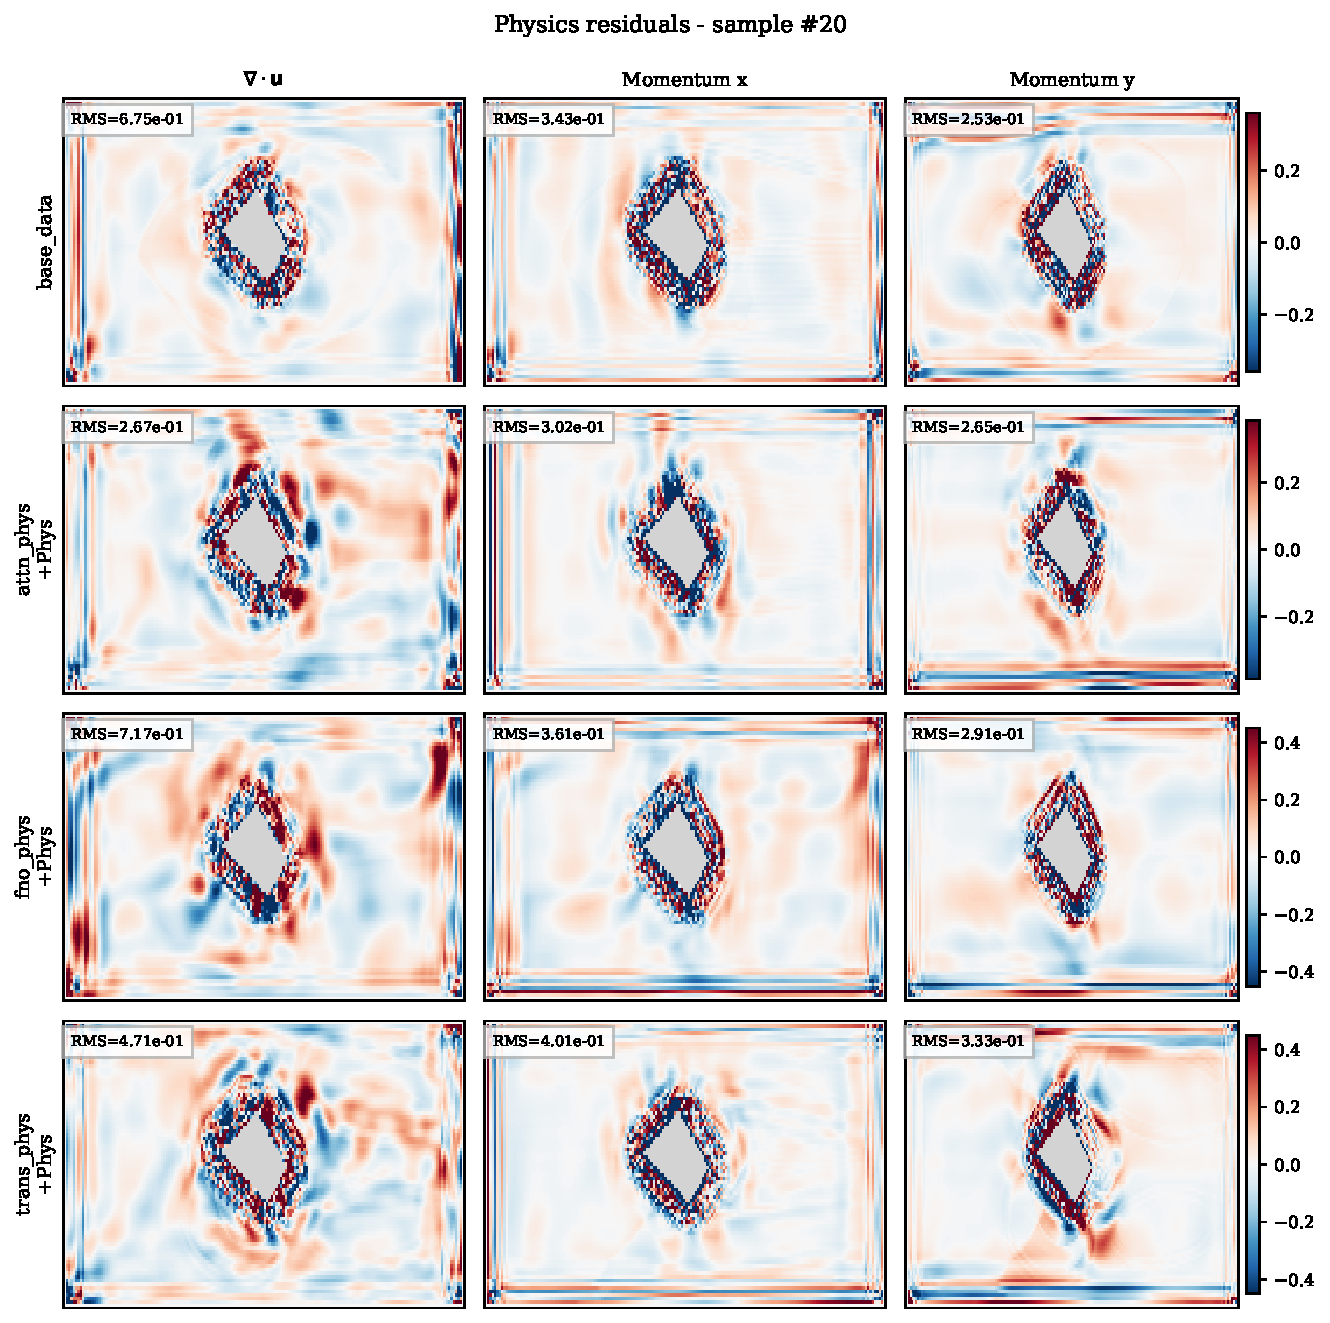
\includegraphics[width=0.95\linewidth]{figures/fig_residuals.pdf}
    \caption{Mappe di residuo di continuita' e quantita' di moto su test set.}
    \label{fig:residuals}
\end{figure}

\section{Discussione}
Nel budget corrente, la componente fisica aiuta in modo chiaro il modello Attention, mentre non porta vantaggi su FNO e Transformer. Questo non implica che FNO e Transformer siano inadatti al problema: indica piuttosto che richiedono una strategia di training piu' lunga o piu' specifica (schedule, pesi PINN, tuning della stabilizzazione).

Le analisi visuali confermano il risultato numerico: UNet-Attention (+phys) mostra un compromesso migliore tra ricostruzione della wake, regolarita' del campo e distribuzione dell'errore su pressione e velocita'.

\section{Conclusioni}
Il confronto svolto in questo coursework mostra che:
\begin{enumerate}
    \item i surrogati neurali consentono forte accelerazione in inferenza,
    \item la loss PINN non e' automaticamente migliorativa: dipende dall'architettura e dal training,
    \item nel setup corrente il miglior modello e' UNet-Attention (+phys),
    \item la valutazione deve includere sia metriche aggregate sia confronto visuale.
\end{enumerate}

Come passi successivi, e' consigliabile estendere il training delle varianti globali (FNO/Transformer) e fare tuning sistematico dei coefficienti $\lambda_c$, $\lambda_m$ e $\lambda_b$.

\end{document}


